% CST EM ANÁLISE E DESENVOLVIMENTO DE SISTEMAS
% INSTITUTO FEDERAL DE SANTA CATARINA - IFSC
% CÂMPUS TUBARÃO

% Modelo de Artigo Científico
% ===============================================================

\documentclass[a4paper, 12pt, oneside]{article}

%%%%%%%%%%%%%%%%%%%%%%%%% PACOTES %%%%%%%%%%%%%%%%%%%%%%%%%%%%%%%%%%

\usepackage[inner = 3cm, outer = 2cm, top = 3cm, bottom= 2cm]{geometry}
\usepackage[utf8]{inputenc}
\usepackage[T1]{fontenc}
\usepackage[brazil]{babel}
\usepackage{hyphenat}
\usepackage{lmodern}
\usepackage{graphicx}
\usepackage{url} % Pacote para formatar URLs
\usepackage{nomencl}
\usepackage{color}
\usepackage{microtype}
\usepackage{lipsum}
\usepackage{amsfonts,amsmath,amssymb}
\usepackage{booktabs}

% Configuração dos parágrafos
\usepackage{indentfirst}
\setlength{\parindent}{1.25cm}

% Configuração do espaçamento
\usepackage{setspace}

% Configuração de alinhamento de texto
\usepackage{ragged2e}

% Configuração de numeração de página
\usepackage{fancyhdr}
\fancyhf{}
\rhead{\thepage}
\cfoot{}
\renewcommand{\headrulewidth}{0pt} % zera linha de cabeçalho
\pagestyle{fancy}
\setlength{\headheight}{15pt}

% Configuração da Fonte
\usepackage{helvet} % Helvetica (similar ao Arial)
\renewcommand{\familydefault}{\sfdefault}

\usepackage[hang,flushmargin]{footmisc} % tirar o espaçamento da nota de rodapé

\usepackage{xcolor}

\makeatletter % para primeiras notas de rodapé
\def\@xfootnote[#1]{%
  \protected@xdef\@thefnmark{#1}%
  \@footnotemark\@footnotetext}
\makeatother

% Formatando Sections
\usepackage{mfirstuc}

\usepackage{titlesec}
\titleformat{\section}{\normalfont\fontsize{12}{12}\bfseries\MakeUppercase}{\thesection}{0.5em}{}

\titleformat{\subsection}{\normalfont\fontsize{12}{12}\bfseries}{\thesubsection}{0.5em}{\capitalisewords}

\titleformat{\subsubsection}{\normalfont\fontsize{12}{12}}{\thesubsubsection}{0.5em}{\capitalisewords}


%PACOTE DE CITAÇÕES
\usepackage[alf]{abntex2cite} % ABNT com bibtex padrão, sem biber

\usepackage{changepage}
\usepackage{ifoddpage}

% Define ambiente quote para citações diretas com mais de 3 linhas
\newenvironment{myquote}{\par\fontsize{10pt}{12pt}\selectfont\begin{adjustwidth}{4cm}{0pt}}{\end{adjustwidth}\par}

% PACOTES ESSENCIAIS
\usepackage{graphicx}
\usepackage{float}
\usepackage{caption}
\usepackage{xurl}
\usepackage{tikz}
\usetikzlibrary{shapes.geometric, arrows.meta, positioning, calc}

% Define o tamanho da fonte para as legendas
\DeclareCaptionFont{mycaptionfont}{\fontsize{10pt}{12pt}\selectfont}

% Aplica o tamanho da fonte definido às legendas de figuras
\captionsetup{font=mycaptionfont}

% Redefine o separador das legendas para travessão (-)
\DeclareCaptionLabelSeparator{myhyphen}{ --- }
\captionsetup{font=mycaptionfont, labelsep=myhyphen}

% Define o espaçamento horizontal da nota de rodapé
\setlength{\footnotemargin}{10pt}

\fancypagestyle{firstpage}{\rhead{\includegraphics[width=\textwidth]{Imagens/Cabecalho.png}}} % Cabeçalho

% Preencha as informações do título, subtítulo, autor e orientador aqui
\newcommand{\titulo}{ARTLINK: DESENVOLVIMENTO DE UMA REDE SOCIAL PARA ARTISTAS E ARTESÃOS}
\newcommand{\autor}{Guilherme Madruga Braga Lessa Martins}
\newcommand{\orientador}{Fabrício Bueno Borges}
\newcommand{\coorientador}{}

\begin{document} %Início do Documento
\thispagestyle{firstpage} % Declara página inicial

\singlespacing % espaçamento simples
\justifying % texto justificado

\newcommand{\citacao}[1]{%
  \begin{list}{}{\setlength{\leftmargin}{4cm}} % ajusta o recuo
  \item \small #1
  \end{list}
}

%%%%%%%%%%%%%%%%%%%%%%%% CONFIG. DO TÍTULO %%%%%%%%%%%%%%%%%%%%%%%%

\vspace*{0.5cm} %Espaçamento Superior do Título
\begin{center} %Inicia a centralização
\textbf{\MakeUppercase{\titulo}}
\end{center} %Finaliza a centralização

%%%%%%%%%%%%%%%%%%%%%%%%% RODAPÉ %%%%%%%%%%%%%%%%%%%%%%%%%%%%%%%%%%

\begin{flushright} %Alinhamento a margem direito

\autor\footnote[*]{Aluno do CST em Análise e Desenvolvimento de Sistemas do IFSC Câmpus Tubarão. E-mail: guilherme.martins@aluno.ifsc.edu.br}

\orientador\footnote[**]{Professor orientador. Professor EBTT de Informática do IFSC Câmpus Tubarão. E-mail: fabricio.borges@ifsc.edu.br}

\end{flushright}

%%%%%%%%%%%%%%%%%%%%% RESUMO E ABSTRACT %%%%%%%%%%%%%%%%%%%%%%%%%%%%%%

\begin{center}
\textbf{\MakeUppercase{Resumo}}
\end{center}

\noindent
O presente artigo descreve o desenvolvimento do Artlink, uma plataforma de rede social voltada a artistas e artesãos brasileiros, concebida como Trabalho de Conclusão de Curso do CST em Análise e Desenvolvimento de Sistemas do IFSC Câmpus Tubarão. O projeto adota a metodologia Design Science Research e foi estruturado em etapas iterativas de levantamento de requisitos, prototipagem, implementação e validação. A solução foi construída com tecnologias modernas: React 18 e TypeScript no \textit{frontend}, Node.js com Express 5, Prisma 6 e PostgreSQL no \textit{backend}, e Cloudinary para armazenamento de imagens na nuvem. O sistema implementa funcionalidades próprias de redes sociais, adaptadas ao contexto criativo: publicação de obras com suporte a múltiplas imagens, sistema de curtidas, comentários, seguidores, \textit{feed} personalizado, mensagens diretas, notificações, catálogos de obras e colaboração entre artistas. O banco de dados foi modelado com 17 entidades relacionais e a API REST conta com 91 \textit{endpoints}. A plataforma encontra-se implantada em ambiente de produção, demonstrando a viabilidade técnica da solução e sua contribuição para a valorização da produção artística e artesanal no ambiente digital.

\noindent \textbf{Palavras-chave:} rede social para artistas; plataforma digital; artesanato; desenvolvimento web; React.

%%%%%%%%%%%%%%%%%%%%%%%%%%%%%% SEÇÕES %%%%%%%%%%%%%%%%%%%%%%%%%%%%%

\section{Introdução}

O crescimento das redes sociais digitais transformou profundamente a maneira como artistas e artesãos promovem e compartilham seu trabalho. No entanto, plataformas generalistas como o Instagram, embora amplamente utilizadas por criadores, não foram projetadas para atender às necessidades específicas do universo artesanal: gestão de portfólios, colaboração entre artesãos, organização de catálogos e construção de uma comunidade voltada à valorização da arte manual.

Nesse contexto, este trabalho propõe o desenvolvimento do \textbf{Artlink}, uma plataforma de rede social desenvolvida especialmente para artistas e artesãos. O sistema combina características típicas de redes sociais --- publicação de obras, curtidas, comentários e sistema de seguidores --- com ferramentas específicas para o setor criativo, como catálogos de obras, convites de colaboração entre artistas e busca por estilos e técnicas mediante \textit{hashtags}. O objetivo é oferecer um espaço digital inclusivo, intuitivo e acessível, capaz de fortalecer as conexões entre criadores e ampliar a visibilidade do artesanato brasileiro.

Embora existam plataformas voltadas ao artesanato, como Etsy e ArtFinder, estas se concentram no comércio eletrônico, deixando de oferecer o componente social e colaborativo que caracteriza comunidades criativas. Ao mesmo tempo, plataformas sociais generalistas carecem de ferramentas de portfólio e colaboração adaptadas ao artesão. O Artlink foi concebido para preencher essa lacuna.

O objetivo geral deste trabalho é desenvolver e implantar em produção uma plataforma de rede social para artistas e artesãos, com funcionalidades que promovam a divulgação, a interação e a colaboração no setor criativo. Para alcançar esse objetivo, foram definidos os seguintes objetivos específicos:

\begin{itemize}
    \item Implementar funcionalidades de rede social, como publicação de obras com imagens, curtidas, comentários, sistema de seguidores e \textit{feed} personalizado;
    \item Desenvolver mecanismos de organização de portfólio, como catálogos de obras e convites de colaboração entre artistas;
    \item Construir uma API REST segura com autenticação via JWT e verificação de e-mail;
    \item Disponibilizar a plataforma em ambiente de produção com infraestrutura inteiramente em nuvem;
    \item Proporcionar uma interface responsiva e acessível para usuários com diferentes níveis de familiaridade tecnológica.
\end{itemize}

\section{Fundamentação Teórica}

\subsection{Redes Sociais Digitais e o Setor Criativo}

As redes sociais digitais são estruturas formadas por atores e suas conexões, constituindo-se como espaços de interação, troca e construção de identidade no ambiente virtual \cite{recuero2009}. Para o setor criativo, essas plataformas representam uma oportunidade de visibilidade e alcance de público que, anteriormente, exigia investimentos significativos em canais tradicionais de divulgação.

Plataformas como Instagram, Pinterest e Behance são amplamente utilizadas por artistas para divulgar seu trabalho. Contudo, essas soluções são de caráter generalista: não oferecem funcionalidades específicas para o contexto artesanal, como gestão de catálogos, colaboração técnica entre criadores ou comunidades organizadas por técnica e estilo. Isso cria uma lacuna no mercado digital, especialmente para artesãos que necessitam de um ambiente simultaneamente social e profissional.

Conforme apontam estudos sobre economia criativa e sociedade em rede, a digitalização do setor artesanal pode ampliar mercados, gerar renda e preservar identidades culturais \cite{castells2003}. Uma plataforma dedicada, portanto, não representa apenas uma solução tecnológica, mas também uma ferramenta de transformação social e econômica para os criadores.

\subsection{Plataformas de Referência para Artistas e Artesãos}

Para compreender o cenário atual e identificar oportunidades de melhoria, foram analisadas duas plataformas de referência com propostas distintas de apoio ao artesanato: Etsy e ArtFinder.

O \textbf{Etsy}, lançado em 2005, é um dos maiores \textit{marketplaces} para produtos artesanais e \textit{vintage} do mundo. A plataforma permite que artesãos criem lojas \textit{online} e vendam diretamente a consumidores finais, oferecendo grande visibilidade global. Contudo, o Etsy se concentra no aspecto comercial, com funcionalidades limitadas de interação social entre criadores \cite{etsy2024}. O modelo de taxas por listagem e por transação pode, ainda, representar um obstáculo para artesãos iniciantes.

O \textbf{ArtFinder}, lançado em 2013, propõe uma abordagem mais curada, voltada à arte e ao artesanato exclusivo. Diferencia-se pela seleção rigorosa dos vendedores, valorizando a exclusividade das obras \cite{artfinder2024}. No entanto, essa barreira de entrada limita o acesso de artesãos em início de carreira, e a plataforma tampouco oferece funcionalidades sociais como seguidores ou \textit{feed} de publicações.

O \textbf{Artlink} foi desenvolvido para preencher as lacunas identificadas nessas plataformas, combinando elementos de rede social com ferramentas de divulgação artística. A Tabela~\ref{tab:comparativo} apresenta um comparativo entre as três plataformas.

\begin{table}[ht]
\centering
\caption{Comparativo entre plataformas para artistas}
\label{tab:comparativo}
\begin{tabular}{|l|c|c|c|}
\hline
\textbf{Funcionalidades} & \textbf{Etsy} & \textbf{ArtFinder} & \textbf{Artlink} \\ \hline
\textit{Feed} social e publicações  & Não  & Não   & Sim   \\ \hline
Sistema de seguidores               & Não  & Não   & Sim   \\ \hline
Mensagens diretas entre usuários    & Parcial & Não  & Sim  \\ \hline
Colaboração entre artistas          & Não  & Não   & Sim   \\ \hline
Catálogos e coleções de obras       & Parcial & Sim  & Sim  \\ \hline
Curtidas e comentários              & Não  & Parcial & Sim  \\ \hline
Notificações de interações          & Sim  & Parcial & Sim  \\ \hline
Busca por \textit{hashtags}         & Parcial & Não  & Sim  \\ \hline
Gestão de estoque e vendas          & Sim  & Sim   & Não   \\ \hline
\end{tabular}
\caption*{Fonte: Elaborado pelo autor (2025)}
\end{table}

O comparativo evidencia que o Artlink se diferencia pelo foco nas interações sociais e na colaboração entre criadores, em detrimento de funcionalidades de \textit{e-commerce} presentes nas demais plataformas analisadas. Essa escolha reflete o objetivo central do sistema: antes de comercializar, conectar.

\section{Desenvolvimento do Sistema}

O \textbf{Artlink} foi desenvolvido com base nos princípios da \textbf{Design Science Research} (DSR), metodologia que orienta a criação e avaliação de artefatos tecnológicos com vistas à resolução de problemas práticos \cite{hevner2004}. O processo foi dividido em quatro etapas iterativas: levantamento de requisitos, prototipagem, implementação e validação.

\subsection{Etapas do Desenvolvimento}

\begin{itemize}
    \item \textbf{Levantamento de requisitos:} Foram identificadas as principais necessidades de artesãos e artistas, como facilidade de cadastro, publicação de obras com imagens, interação com outros criadores e organização de portfólios. Os requisitos foram documentados e priorizados segundo sua relevância para o público-alvo.

    \item \textbf{Prototipagem:} As interfaces foram prototipadas no \textbf{Figma}, com foco na experiência do usuário (UX) e na acessibilidade. O \textit{design} priorizou um \textit{layout} responsivo e intuitivo, adequado tanto para computadores quanto para dispositivos móveis.

    \item \textbf{Implementação:} O desenvolvimento foi realizado no \textit{Visual Studio Code} (VS Code), utilizando o ecossistema JavaScript/TypeScript em ambas as camadas da aplicação. A organização modular do código garantiu escalabilidade e facilidade de manutenção.

    \item \textbf{Validação:} O sistema foi submetido a testes de integração e de usabilidade. A plataforma foi implantada em produção no serviço de hospedagem Render.com, validando sua operação em ambiente real.
\end{itemize}

\subsection{Arquitetura e Tecnologias Utilizadas}

O Artlink adota uma arquitetura cliente-servidor, composta por um \textit{frontend} baseado em SPA (\textit{Single Page Application}) e uma API REST no \textit{backend}. Essa separação permite independência entre as camadas, facilita a manutenção e possibilita o eventual desenvolvimento de clientes nativos (aplicativo móvel) sem alterações no servidor.

A Tabela~\ref{tab:tecnologias} apresenta as principais tecnologias utilizadas no desenvolvimento.

\begin{table}[ht]
\centering
\caption{Tecnologias utilizadas no desenvolvimento do Artlink}
\label{tab:tecnologias}
\begin{tabular}{lll}
\toprule
\textbf{Camada} & \textbf{Tecnologia} & \textbf{Versão} \\
\midrule
\textit{Frontend} & React       & 18.2.0 \\
\textit{Frontend} & TypeScript  & 5.9.3  \\
\textit{Frontend} & Vite        & 5.1.0  \\
\textit{Frontend} & React Router & 7.9.4 \\
\textit{Frontend} & Axios       & 1.12.2 \\
\textit{Frontend} & SASS        & 1.93.2 \\
\textit{Backend}  & Node.js + Express & 5.1.0 \\
\textit{Backend}  & TypeScript  & 5.9.2  \\
\textit{Backend}  & Prisma ORM  & 6.15.0 \\
\textit{Backend}  & bcrypt      & 6.0.0  \\
\textit{Backend}  & jsonwebtoken & 9.0.3 \\
Banco de dados    & PostgreSQL (Supabase) & -- \\
Armazenamento     & Cloudinary  & 2.10.0 \\
E-mail            & Resend API  & 6.12.3 \\
Hospedagem        & Render.com  & --     \\
\bottomrule
\end{tabular}
\caption*{Fonte: Elaborado pelo autor (2025)}
\end{table}

O \textbf{React} foi escolhido para o \textit{frontend} por sua abordagem baseada em componentes reutilizáveis e sua ampla adoção pela comunidade \cite{react2024}. O \textbf{TypeScript} foi adotado em ambas as camadas por oferecer tipagem estática, reduzindo erros em tempo de execução e melhorando a manutenibilidade do código \cite{typescript2024}. No \textit{backend}, o \textbf{Express 5} gerencia as rotas e \textit{middlewares} da API REST, enquanto o \textbf{Prisma} atua como ORM, abstraindo as operações de banco de dados e garantindo segurança nas consultas \cite{prisma2024}.

\begin{figure}[!ht]
\caption{Arquitetura geral do sistema Artlink}
\centering
\begin{tikzpicture}[
  box/.style  = {rectangle, rounded corners=5pt, draw=black!70, thick,
                 text centered, font=\small\sffamily,
                 minimum height=1.5cm, minimum width=3.2cm, align=center},
  ext/.style  = {rectangle, rounded corners=5pt, draw=black!50,
                 text centered, font=\small\sffamily,
                 minimum height=1cm, minimum width=3cm, align=center},
  arr/.style  = {<->, >=Stealth, thick, black!70},
  arr1/.style = {->, >=Stealth, thick, black!50},
  lbl/.style  = {font=\scriptsize\sffamily, fill=white, inner sep=1pt},
]
  \node[box, fill=blue!15] (frontend) at (0,0) {
    \textbf{Frontend}\\[2pt]
    React 18 + TypeScript\\
    Vite + React Router
  };
  \node[box, fill=orange!15] (backend) at (5.2,0) {
    \textbf{Backend}\\[2pt]
    Node.js + Express 5\\
    TypeScript + Prisma 6
  };
  \node[box, fill=green!15] (banco) at (10.4,0) {
    \textbf{PostgreSQL}\\[2pt]
    Supabase\\
    (17 entidades)
  };
  \node[ext, fill=purple!10] (cloudinary) at (5.2,-2.6) {
    \textbf{Cloudinary}\\
    \scriptsize Armazenamento de imagens
  };
  \node[ext, fill=yellow!20] (resend) at (5.2,2.6) {
    \textbf{Resend API}\\
    \scriptsize Envio de e-mails
  };

  \draw[draw=blue!40, dashed, thick, rounded corners=8pt]
    ($(frontend.north west)+(-0.4,0.35)$) rectangle ($(backend.south east)+(0.4,-0.35)$);
  \node[font=\scriptsize\sffamily, text=blue!60]
    at ($(frontend.north west)!0.5!(backend.north east)+(0,0.5)$) {Render.com};

  \draw[arr]  (frontend) -- node[lbl, above] {API REST} node[lbl, below] {HTTPS/JSON} (backend);
  \draw[arr]  (backend)  -- node[lbl, above] {Prisma ORM} node[lbl, below] {SSL} (banco);
  \draw[arr1] (backend)  -- node[lbl, right] {upload / CDN} (cloudinary);
  \draw[arr1] (backend)  -- node[lbl, right] {SMTP} (resend);
\end{tikzpicture}\\[6pt]
{\small Fonte: Elaborado pelo autor (2025)}
\label{fig:arquitetura}
\end{figure}

\subsection{Modelagem do Banco de Dados}

O banco de dados foi modelado de forma relacional no PostgreSQL, utilizando o Prisma como ORM para definição do \textit{schema} e geração de migrações. O modelo conta com 17 entidades, cobrindo desde o gerenciamento de usuários até o controle de notificações e mensagens diretas. A Tabela~\ref{tab:entidades} apresenta as principais entidades com seus campos e funções no sistema.

\begin{table}[ht]
\centering
\caption{Principais entidades do banco de dados do Artlink}
\label{tab:entidades}
\begin{tabular}{lp{5.5cm}p{4cm}}
\toprule
\textbf{Entidade} & \textbf{Campos Principais} & \textbf{Descrição} \\
\midrule
\texttt{Usuario}         & id, nome, username, email, senha, bio, fotoPerfil, fotoCapa, emailVerificado & Artistas e usuários da plataforma \\
\texttt{Post}            & id, usuarioId, titulo, descricao, imagens, tags, visualizacoes & Publicações de obras artísticas \\
\texttt{Catalogo}        & id, usuarioId, nome, descricao, capa & Coleções e portfólios de obras \\
\texttt{Curtida}         & id, usuarioId, postId, data & Curtidas em publicações \\
\texttt{Comentario}      & id, usuarioId, postId, conteudo, data & Comentários em publicações \\
\texttt{Seguidor}        & seguidorId, seguidoId, data & Relacionamento de seguidores \\
\texttt{Mensagem}        & id, remetenteId, destinatarioId, conteudo, imagem, dataEnvio, status & Mensagens diretas entre usuários \\
\texttt{Notificacao}     & id, usuarioId, tipo, remetenteId, postId, lida & Notificações de interações \\
\texttt{PostColaboracao} & postId, usuarioId, status & Convites de colaboração em obras \\
\texttt{PostSalvo}       & id, usuarioId, postId, salvadoEm & Publicações salvas pelo usuário \\
\texttt{Visualizacao}    & usuarioId, postId, criadoEm & Log de visualizações de \textit{posts} \\
\bottomrule
\end{tabular}
\caption*{Fonte: Elaborado pelo autor (2025)}
\end{table}

A entidade \texttt{Notificacao} utiliza um \textit{enum} (\texttt{TipoNotificacao}) com os valores \texttt{curtida}, \texttt{comentario}, \texttt{seguindo}, \texttt{colaboracao}, \texttt{colaboracao\_catalogo} e \texttt{mensagem}, permitindo a categorização precisa de cada evento gerado pelo sistema.

\begin{figure}[!ht]
\caption{Diagrama simplificado do modelo relacional do banco de dados}
\centering
\begin{tikzpicture}[
  ent/.style = {rectangle, draw=black!70, thick, rounded corners=2pt,
                font=\scriptsize\sffamily,
                minimum width=2.6cm, minimum height=0.9cm, align=center},
  rel/.style = {->, >=Stealth, semithick, black!55},
  lbl/.style = {font=\tiny\sffamily, fill=white, inner sep=1pt},
]
  \node[ent] (usuario)    at (0,   0)   {\textbf{Usuario}\\nome, username, email};
  \node[ent] (post)       at (4.5, 0)   {\textbf{Post}\\titulo, imagens, tags};
  \node[ent] (catalogo)   at (0,   2.2) {\textbf{Catalogo}\\nome, descricao};
  \node[ent] (curtida)    at (8,   1.2) {\textbf{Curtida}\\usuarioId, postId};
  \node[ent] (comentario) at (8,  -1.2) {\textbf{Comentario}\\postId, conteudo};
  \node[ent] (seguidor)   at (-3.5, 0)  {\textbf{Seguidor}\\seguidorId, seguidoId};

  \draw[rel] (usuario) -- node[lbl,above]{1:N} (post);
  \draw[rel] (usuario) -- node[lbl,right]{1:N} (catalogo);
  \draw[rel] (post)    -- node[lbl,above,sloped]{1:N} (curtida);
  \draw[rel] (post)    -- node[lbl,below,sloped]{1:N} (comentario);
  \draw[rel] (usuario) -- node[lbl,above]{N:N} (seguidor);
\end{tikzpicture}\\[6pt]
{\small Fonte: Elaborado pelo autor (2025)}
\label{fig:diagrama_banco}
\end{figure}

\subsection{Diagramas UML}

O diagrama de classes (Figura~\ref{fig:classes}) apresenta as principais entidades do sistema e seus relacionamentos, representados no estilo UML com atributos e multiplicidades. O diagrama de casos de uso (Figura~\ref{fig:casos_uso}) descreve as interações entre os dois perfis de atores da plataforma --- Visitante e Usuário Autenticado --- e as funcionalidades disponíveis para cada um.

\begin{figure}[!ht]
\caption{Principais classes do sistema Artlink com atributos e tipos}
\centering
\small
\begin{tabular}{@{}p{2.3cm}lp{1.6cm}@{\hspace{1cm}}p{2.3cm}lp{1.6cm}@{}}
\toprule
\textbf{Classe} & \textbf{Atributo} & \textbf{Tipo} &
\textbf{Classe} & \textbf{Atributo} & \textbf{Tipo} \\
\midrule
\texttt{Usuario}     & id           & Int       & \texttt{Post}       & id            & Int       \\
                     & nome         & String    &                     & titulo        & String    \\
                     & username     & String    &                     & imagens       & String[]  \\
                     & email        & String    &                     & tags          & String[]  \\
                     & fotoPerfil   & String?   &                     & visualizacoes & Int       \\
\addlinespace[5pt]
\texttt{Catalogo}    & id           & Int       & \texttt{Curtida}    & id            & Int       \\
                     & nome         & String    &                     & usuarioId     & Int       \\
                     & descricao    & String?   &                     & postId        & Int       \\
                     & capa         & String?   &                     & data          & DateTime  \\
\addlinespace[5pt]
\texttt{Seguidor}    & seguidorId   & Int       & \texttt{Comentario} & id            & Int       \\
                     & seguidoId    & Int       &                     & postId        & Int       \\
                     & data         & DateTime  &                     & conteudo      & String    \\
\addlinespace[5pt]
\texttt{Mensagem}    & remetenteId  & Int       & \texttt{Notificacao}& usuarioId     & Int       \\
                     & conteudo     & String?   &                     & tipo          & Enum      \\
                     & status       & Enum      &                     & lida          & Boolean   \\
\bottomrule
\end{tabular}
\caption*{Fonte: Elaborado pelo autor (2025)}
\label{fig:classes}
\end{figure}

\begin{figure}[!ht]
\caption{Diagrama de casos de uso do Artlink}
\centering
\begin{tikzpicture}[font=\scriptsize\sffamily]
  \draw[rounded corners=4pt] (0.5,-5) rectangle (8,4.2);
  \node[font=\small\sffamily\bfseries] at (4.25, 3.9) {Artlink};
  \draw[dashed, black!30] (0.7, 1.3) -- (7.8, 1.3);
  \node[font=\tiny\sffamily\itshape, text=black!40] at (4.25, 1.1) {requer autenticação};

  \node[draw, ellipse, align=center] (vis) at (-1.3,  2.5) {Visitante};
  \node[draw, ellipse, align=center] (aut) at (-1.3, -1.8) {Usuário\\Autenticado};
  \draw[->, dashed] (aut) -- (vis);

  \node[draw, ellipse, minimum width=3.4cm] (u1) at (4.25, 3.5) {Visualizar perfis};
  \node[draw, ellipse, minimum width=3.4cm] (u2) at (4.25, 2.6) {Buscar artistas};
  \node[draw, ellipse, minimum width=3.4cm] (u3) at (4.25, 1.7) {Navegar por hashtags};
  \node[draw, ellipse, minimum width=3.4cm] (a1) at (4.25,  0.5) {Publicar obra};
  \node[draw, ellipse, minimum width=3.4cm] (a2) at (4.25, -0.4) {Criar catálogo};
  \node[draw, ellipse, minimum width=3.4cm] (a3) at (4.25, -1.3) {Curtir e comentar};
  \node[draw, ellipse, minimum width=3.4cm] (a4) at (4.25, -2.2) {Seguir artista};
  \node[draw, ellipse, minimum width=3.4cm] (a5) at (4.25, -3.1) {Enviar mensagem};
  \node[draw, ellipse, minimum width=3.4cm] (a6) at (4.25, -4.0) {Gerenciar perfil};

  \draw (vis.east) -- (u1.west); \draw (vis.east) -- (u2.west); \draw (vis.east) -- (u3.west);
  \draw (aut.east) -- (a1.west); \draw (aut.east) -- (a2.west); \draw (aut.east) -- (a3.west);
  \draw (aut.east) -- (a4.west); \draw (aut.east) -- (a5.west); \draw (aut.east) -- (a6.west);
\end{tikzpicture}\\[6pt]
{\small Fonte: Elaborado pelo autor (2025)}
\label{fig:casos_uso}
\end{figure}

\subsection{Funcionalidades Implementadas}

O Artlink foi desenvolvido com um conjunto abrangente de funcionalidades organizadas em módulos. A API REST conta com 91 \textit{endpoints} distribuídos em 17 grupos funcionais. As principais funcionalidades da plataforma são:

\begin{itemize}
    \item \textbf{Autenticação e segurança:} Cadastro com verificação de e-mail (link de confirmação com validade de 24 horas via Resend API), \textit{login} com e-mail ou nome de usuário, recuperação de senha com código temporário e geração de tokens via JWT;
    \item \textbf{Publicações:} Criação de \textit{posts} com múltiplas imagens armazenadas no Cloudinary, título, descrição, \textit{tags} e convites de colaboração para outros artistas;
    \item \textbf{Interações sociais:} Curtidas em publicações, comentários, sistema de seguidores (\textit{follow/unfollow}) e \textit{feed} personalizado exibindo as publicações dos usuários seguidos;
    \item \textbf{Catálogos:} Criação e gerenciamento de coleções de obras com suporte a imagens adicionais e colaboração entre artistas;
    \item \textbf{Mensagens diretas:} Sistema de DM (\textit{Direct Message}) com envio de texto e imagens, edição, exclusão individual, arquivamento de conversas e solicitações de mensagem;
    \item \textbf{Notificações:} Notificações geradas automaticamente para curtidas, comentários, novos seguidores, convites de colaboração e mensagens recebidas;
    \item \textbf{Busca e descoberta:} Pesquisa de usuários e publicações por texto, navegação por \textit{hashtags} e sugestões de artistas para novos usuários com \textit{feed} vazio;
    \item \textbf{Perfis personalizados:} Foto de perfil, foto de capa, biografia, cidade, configuração de tema claro/escuro e botão de cópia de \textit{link} do perfil;
    \item \textbf{Controle de visualizações:} Registro de visualizações únicas por usuário com deduplicação via \texttt{localStorage} para visitantes não autenticados.
\end{itemize}

\subsection{Implantação e Infraestrutura}

O Artlink foi projetado para operar integralmente em serviços de nuvem, garantindo escalabilidade e disponibilidade. A infraestrutura de produção é composta pelos seguintes serviços:

\begin{itemize}
    \item \textbf{Render.com:} Hospedagem do servidor Node.js. O \textit{build} do \textit{frontend} React é compilado estaticamente com Vite e servido pelo próprio Express em produção, resultando em um único processo de servidor;
    \item \textbf{Supabase:} Banco de dados PostgreSQL gerenciado, com conexão segura via SSL e variáveis de ambiente;
    \item \textbf{Cloudinary:} Armazenamento e entrega de imagens com CDN global, utilizado para fotos de perfil, capas, imagens de \textit{posts} e catálogos;
    \item \textbf{Resend:} Serviço de envio transacional de e-mails, utilizado para envio de links de verificação de conta e redefinição de senha.
\end{itemize}

O fluxo de \textit{build} é automatizado: o comando \texttt{npm run build} instala as dependências do \textit{frontend}, compila o React com Vite, gera o cliente Prisma, transpila o TypeScript do \textit{backend} e copia os arquivos estáticos para o diretório de distribuição, resultando em um único artefato pronto para produção.

\section{Resultados e Discussão}

O desenvolvimento do Artlink resultou em uma plataforma funcional implantada em ambiente de produção, acessível publicamente pelo endereço \url{https://artlink-iwq1.onrender.com}. Todos os objetivos específicos definidos no início do trabalho foram alcançados.

Do ponto de vista técnico, o sistema conta com uma API REST composta por 91 \textit{endpoints} organizados em 17 grupos funcionais, e um banco de dados relacional com 17 entidades. A separação entre \textit{frontend} (React + Vite) e \textit{backend} (Node.js + Express) garantiu uma arquitetura de fácil manutenção e extensão futura. O uso de TypeScript em ambas as camadas contribuiu para a redução de erros e para a legibilidade do código ao longo do desenvolvimento.

A autenticação implementada com JWT e verificação de e-mail via Resend demonstrou-se robusta, impedindo acessos não autorizados e garantindo a integridade das contas cadastradas. O armazenamento de imagens no Cloudinary eliminou a necessidade de gerenciar espaço em disco no servidor, tornando o sistema mais escalável.

O conjunto de funcionalidades sociais --- seguidores, \textit{feed} personalizado, curtidas, comentários e mensagens diretas --- posiciona o Artlink como uma solução diferenciada frente às plataformas analisadas. Conforme o comparativo da Tabela~\ref{tab:comparativo}, o Artlink é a única das três plataformas que integra funcionalidades de rede social com ferramentas voltadas ao contexto artesanal.

O sistema de notificações e o mecanismo de deduplicação de visualizações representam diferenciais técnicos relevantes, contribuindo para métricas precisas de engajamento e para uma experiência de uso mais fluida. A interface responsiva, desenvolvida com React e SASS, demonstrou funcionar adequadamente em diferentes tamanhos de tela, atendendo ao requisito de acessibilidade previsto nos objetivos do projeto.

A Figura~\ref{fig:tela_feed} apresenta a interface do \textit{feed} principal da plataforma, onde são exibidas as publicações dos artistas seguidos pelo usuário.

\begin{figure}[!ht]
\caption{Interface do \textit{feed} principal do Artlink}
\centering
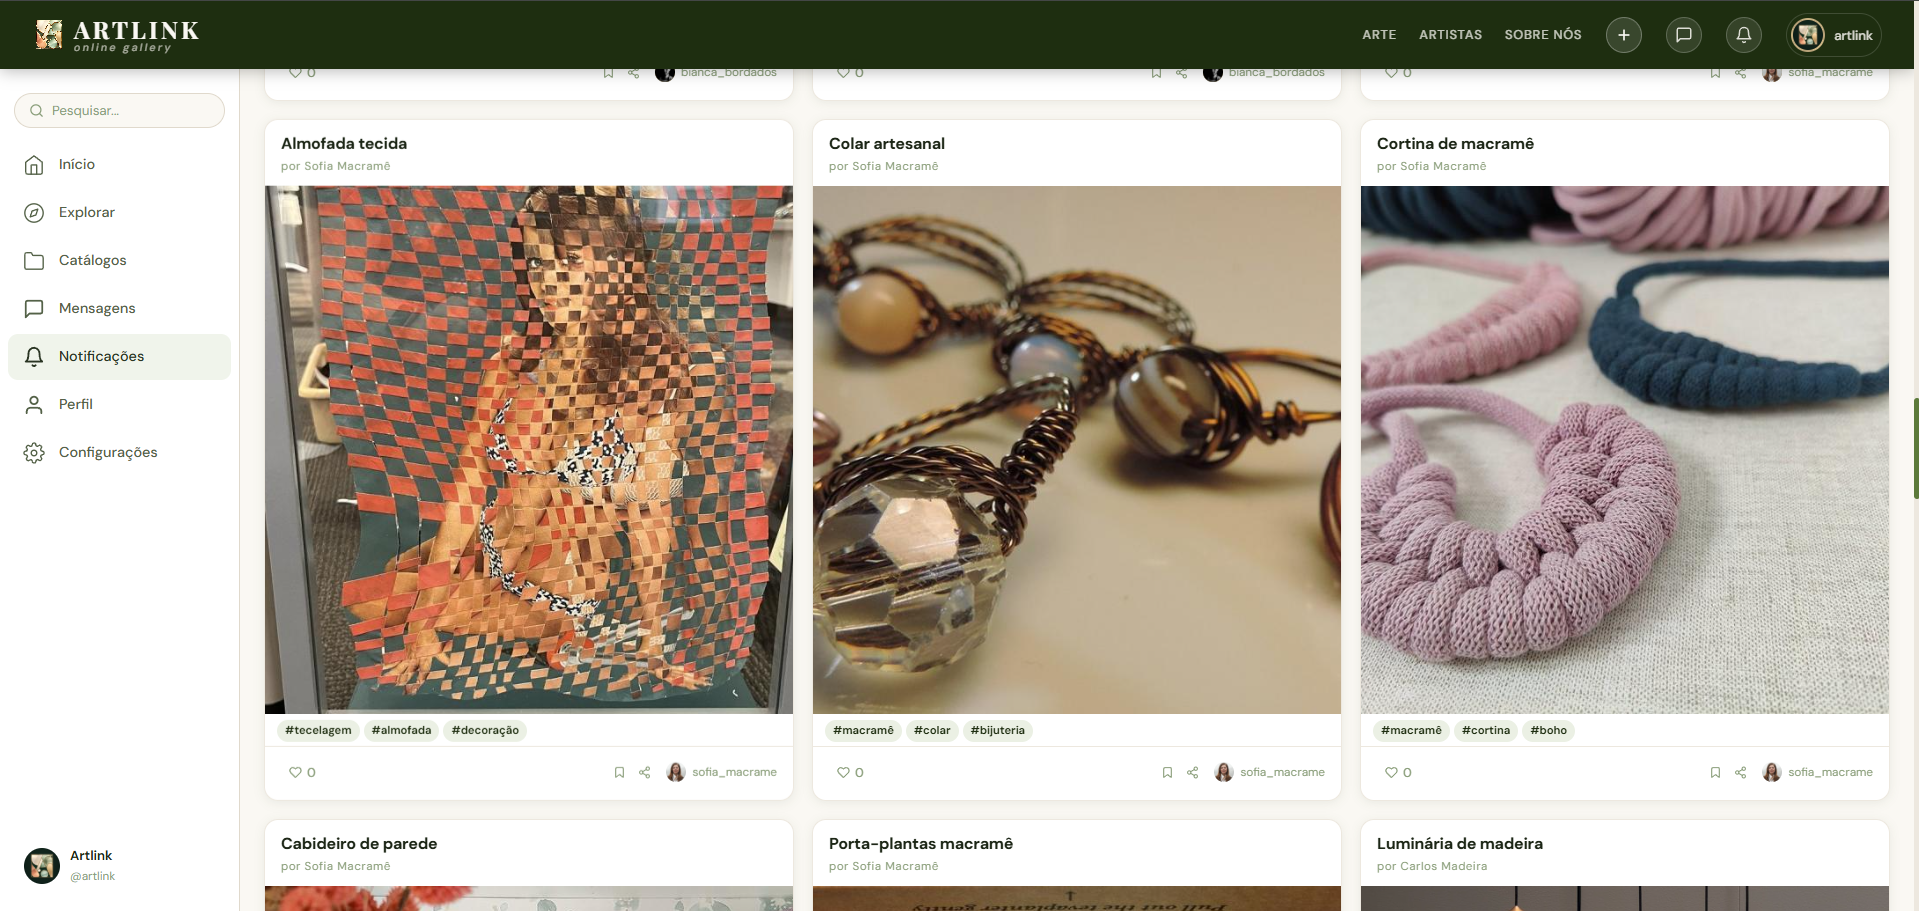
\includegraphics[width=0.75\textwidth]{Imagens/tela_feed_artlink.png}\\
{\small Fonte: Captura de tela elaborada pelo autor (2025)}
\label{fig:tela_feed}
\end{figure}

\section{Considerações Finais}

Este trabalho apresentou o desenvolvimento do \textbf{Artlink}, uma plataforma de rede social para artistas e artesãos construída com tecnologias modernas do ecossistema JavaScript/TypeScript. O sistema foi concebido para preencher uma lacuna identificada no mercado digital: a ausência de uma plataforma que combine as funcionalidades de rede social com ferramentas específicas para o setor criativo, como catálogos de obras e colaboração entre artistas.

Os objetivos propostos foram integralmente alcançados. A plataforma foi desenvolvida, testada e implantada em produção, com todas as funcionalidades planejadas em operação. A adoção do Design Science Research como metodologia mostrou-se adequada para guiar o processo, permitindo ciclos iterativos de validação que aprimoraram continuamente a solução. A escolha por uma arquitetura cliente-servidor com API REST e SPA possibilitou a entrega de uma experiência de uso fluida, comparável à de plataformas sociais consolidadas.

Como trabalhos futuros, destacam-se as seguintes possibilidades de evolução:

\begin{itemize}
    \item Desenvolvimento de aplicativo nativo para dispositivos móveis (iOS e Android);
    \item Integração de funcionalidades de \textit{e-commerce}, permitindo a comercialização de obras diretamente pela plataforma;
    \item Implementação de sistema de eventos e exposições virtuais para artistas;
    \item Adição de recursos de inteligência artificial para recomendação de obras e artistas com base no comportamento do usuário.
\end{itemize}

O Artlink representa uma contribuição concreta para a valorização do artesanato e da arte no ambiente digital brasileiro, oferecendo aos criadores um espaço próprio para se conectar, compartilhar e crescer.

%%%%%%%%%%%%%%%%%%%%%%%%%% REFERÊNCIAS %%%%%%%%%%%%%%%%%%%%%%%%%%%%%%%%

\bibliography{referencias}

%%%%%%%%%%%%%%%%%%%%%%%%%% APÊNDICES %%%%%%%%%%%%%%%%%%%%%%%%%%%%%%%%
\clearpage
\section*{Apêndice A --- Capturas de Tela da Plataforma Artlink}

As figuras a seguir apresentam capturas de tela das principais interfaces do Artlink em ambiente de produção, incluindo a tela de cadastro, perfil do artista, publicação de obra, catálogos, mensagens diretas e painel de notificações.

[Inserir capturas de tela da plataforma em produção.]

%%%%%%%%%%%%%%%%%%%%%%%%%% ANEXOS %%%%%%%%%%%%%%%%%%%%%%%%%%%%%%%%

\clearpage
\section*{Anexo A --- Schema Completo do Banco de Dados}

O \textit{schema} completo do banco de dados do Artlink, contendo todas as 17 entidades definidas no arquivo \texttt{schema.prisma}, encontra-se disponível no repositório do projeto no GitHub.

\end{document}
